\documentclass{article}
\usepackage[utf8]{inputenc}
\usepackage{t1enc}
\usepackage{geometry}
 \geometry{
 a4paper,
 total={210mm,297mm},
 left=20mm,
 right=20mm,
 top=20mm,
 bottom=20mm,
 }
\usepackage{amsmath}
\usepackage{amssymb}
\usepackage{pgf,tikz}
\usetikzlibrary{arrows}
\frenchspacing
\usepackage{fancyhdr}
\pagestyle{fancy}
\lhead{Urbán János tanár úr feladatsorai}
\chead{C08/7./1.}
\rhead{Függvények}
\lfoot{}
\cfoot{\thepage}
\rfoot{}

\usepackage{enumitem}
\usepackage{multicol}
\usepackage{calc}
\newenvironment{abc}{\begin{enumerate}[label=\textit{\alph*})]}{\end{enumerate}}
\newenvironment{abc2}{\begin{enumerate}[label=\textit{\alph*})]\begin{multicols}{2}}{\end{multicols}\end{enumerate}}
\newenvironment{abc3}{\begin{enumerate}[label=\textit{\alph*})]\begin{multicols}{3}}{\end{multicols}\end{enumerate}}
\newenvironment{abc4}{\begin{enumerate}[label=\textit{\alph*})]\begin{multicols}{4}}{\end{multicols}\end{enumerate}}
\newenvironment{abcn}[1]{\begin{enumerate}[label=\textit{\alph*})]\begin{multicols}{#1}}{\end{multicols}\end{enumerate}}
\setlist[enumerate,1]{listparindent=\labelwidth+\labelsep}

\newcommand{\degre}{\ensuremath{^\circ}}
\newcommand{\tg}{\mathop{\mathrm{tg}}\nolimits}
\newcommand{\ctg}{\mathop{\mathrm{ctg}}\nolimits}
\newcommand{\arc}{\mathop{\mathrm{arc}}\nolimits}
\renewcommand{\arcsin}{\arc\sin}
\renewcommand{\arccos}{\arc\cos}
\newcommand{\arctg}{\arc\tg}
\newcommand{\arcctg}{\arc\ctg}
 \newcommand{\sgn}{\operatorname{sgn}}

\parskip 8pt
\begin{document}

\section*{Függvények}

\subsection*{2008.12.09. -- Függvények}
\begin{enumerate}
\item Ábrázoljuk a következő függvényeket:
\begin{abc4}
\item $f(x) = 2x-1$;
\item $g(x) = x+3$;
\item $h(x) = -x+2$;
\item $k(x) = -\frac{1}{2}x+2$.
\end{abc4}
\item Ábrázoljuk a következő függvényeket:
\begin{abc4}
\item $x\mapsto |x|$;
\item $x\mapsto |x-2|$;
\item $x\mapsto |x+1|$;
\item $x\mapsto |x+2|+|x-3|$.
\end{abc4}
\item Ábrázoljuk a következő függvényeket:
\begin{abc4}
\item $x\mapsto 2|x|$;
\item $x\mapsto |2x|$;
\item $x\mapsto |x|-2$;
\item $x\mapsto |x-2|-|x-3|$.
\end{abc4}

\end{enumerate}

\subsection*{2008.12.10.}
\begin{enumerate}
\item Ábrázoljuk:
\begin{abc3}
\item $x\mapsto |2x-1|$;
\item $x\mapsto |x-1|-|x+3|$;
\item $x\mapsto |\frac12 x+1|$;
\item $x\mapsto |3x-2|$;
\item $x\mapsto \frac{|x|}{2}$;
\item $x\mapsto |2x-1|+|x+1|$;
\item $x\mapsto \left||x|-2\right|$;
\item $x\mapsto \left||x-2|-1\right|$;
\item $x\mapsto ||||x|-3|-2|-1|$.
\end{abc3}
\end{enumerate}

\subsection*{2008.12.11.}
\begin{enumerate}
\item Ábrázoljuk a derékszögű koordináta-rendszerben azokat a 
$P(x;y)$ pontokat, amelyeknek koordinátáira igaz a következő összefüggés:
\begin{abc3}
\item $x\ge y$;
\item $|x|\ge |y|$;
\item $|x-1|\le 1$;
\item $|x+1|\ge 1$;
\item $|x+1|+|y-1|\le 2$.
\end{abc3}
\item Ábrázoljuk a következő függvényeket:
\begin{abc3}
\item $x\mapsto |||x-1|-2|-3|$;
\item $x\mapsto |x+2|+|x|+|x-3|$;
\item $x\mapsto ||x+3|-|x-2||$;
\item $x\mapsto x-|x|$;
\item $x\mapsto |2|x|-x|$.
\end{abc3}

\end{enumerate}

\subsection*{2008.12.16.}
Ábrázoljuk a következő függvényeket:
\begin{enumerate}
\item $x\mapsto ||x-3|-|x+1||$;
\item $x\mapsto ||x|+|x-2|-|x+1|$;
\item $x\mapsto |x+2|+|x|+|x-3|$;
\item $x\mapsto |x+3|+|x+1|+|x-2|+|x-4|$;
\item $x\mapsto |2x-1|-|2x+1|$;
\item $x\mapsto ||x-3|-|x|-|x+1||$;
\item $x\mapsto |3|x|-|x-1||$;
\item $x\mapsto |2x-3|+|2x-4|$.
\end{enumerate}

\subsection*{2008.12.18.}
\begin{enumerate}
\item Öt gyufásdobozra ráírtuk a bennük található gyufaszálak számát. A gyufásdobozok egy kör kerülete mentén helyezkednek el. Szomszédos dobozokból 
lehet átrakni egymásba gyufaszálakat. A cél az, hogy minden gyufásdobozban azonos számú gyufaszál legyen és az összes átrakott gyufaszálak száma a lehető legkevesebb legyen.
\begin{center}
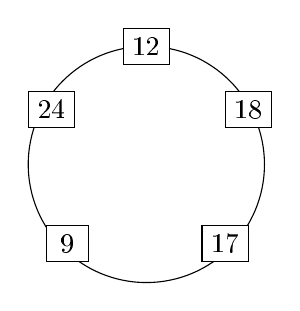
\begin{tikzpicture}[x=1.0cm,y=1.0cm, fill=white]
\draw(2,2) circle (1.5cm);
\draw (2,3.5) node[fill=white,draw] {12};
\draw (3.3,2.7) node[fill=white,draw] {18};
\draw (0.8,2.7) node[fill=white,draw] {24};
\draw (1,1) node[fill=white,draw] {\,9\,};
\draw (3,1) node[fill=white,draw] {17};
\end{tikzpicture}
\end{center}
\item Az 1. feladatban megfogalmazott célt kell elérni, ha a gyufásdobozokban
a gyufaszálak száma:
\begin{abc2}
\item ~

\begin{center}
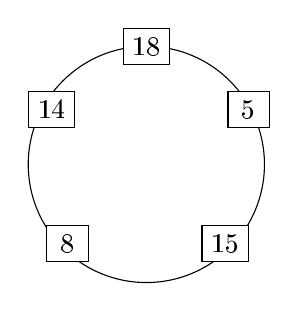
\begin{tikzpicture}[x=1.0cm,y=1.0cm, fill=white]
\draw(2,2) circle (1.5cm);
\draw (2,3.5) node[fill=white,draw] {18};
\draw (3.3,2.7) node[fill=white,draw] {\,5\,};
\draw (0.8,2.7) node[fill=white,draw] {14};
\draw (1,1) node[fill=white,draw] {\,8\,};
\draw (3,1) node[fill=white,draw] {15};
\end{tikzpicture}
\end{center}

\item ~

\begin{center}
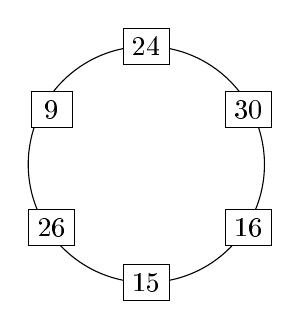
\begin{tikzpicture}[x=1.0cm,y=1.0cm, fill=white]
\draw(2,2) circle (1.5cm);
\draw (2,3.5) node[fill=white,draw] {24};
\draw (3.3,2.7) node[fill=white,draw] {30};
\draw (0.8,2.7) node[fill=white,draw] {\,9\,};
\draw (3.3,1.2) node[fill=white,draw] {16};
\draw (0.8,1.2) node[fill=white,draw] {26};
\draw (2,0.5) node[fill=white,draw] {15};
\end{tikzpicture}
\end{center}

\end{abc2}
\end{enumerate}

\subsection*{2009.01.06. -- Ismétlő feladatok}
Ábrázoljuk a következő függvényeket:
\begin{enumerate}
\item $x\mapsto ||x+2|-|x-1||$;
\item $x\mapsto |x+3|+|x|+|x-4|$;
\item $x\mapsto |2|x|-|x+1||$;
\item $x\mapsto |x-1|+x+|x+1|$;
\item $x\mapsto |2x-|x-1|-|x+1||$.
\end{enumerate}


\subsection*{2009.01.07. -- Függvények}
Ábrázoljuk a következő függvényeket:
\begin{enumerate}
\item $x\mapsto ||x-2|-1|-1$;
\item $x\mapsto |2x-1|-|2x+1|$;
\item $x\mapsto ||x+2|-|x|-|x-2||$;
\item $x\mapsto |x+3|+|x|+|x-2|$;
\item $x\mapsto |2x|-|x|+|x-1|$.
\end{enumerate}


\subsection*{2009.01.12.}
Ábrázoljuk:
\begin{enumerate}
\item $x\mapsto [2x]$;
\item $x\mapsto [x-1]$;
\item $x\mapsto [x]+[-x]$;
\item $x\mapsto [~|x|~]$;
\item $x\mapsto \big|[x]\big|$;
\item $x\mapsto x\cdot [x]$;
\item $x\mapsto \dfrac{x}{[x]}$, $x<0$ vagy $x\ge 1$.
\end{enumerate}


\subsection*{2009.01.14.}
\begin{enumerate}
\item Ábrázoljuk:
\begin{abc2}
\item $x\mapsto \dfrac{x}{[x]}$, $x<0$ vagy $x\ge 1$;
\item $x\mapsto x-[x]$;
\item $x\mapsto [2x]-[x]$;
\item $x\mapsto [x]\cdot[-x]$;
\item $x\mapsto [2x]-2[x]$.
\end{abc2}
\item Hol vannak a síkon azok a $P(x;y)$ pontok, amelyeknek koordinátáira teljesül:
\begin{abc3}
\item $x=[y]$;
\item $[x]=y$;
\item $[x]=[y]$?
\end{abc3}
\end{enumerate}


\subsection*{2009.01.15.}
\begin{enumerate}
\item Ábrázoljuk a következő függvényeket:
\begin{abc3}
\item $x\mapsto x\cdot \left[\dfrac{1}{x}\right]$, ha $x\ne 0$;
\item $x\mapsto [x]+\left[x+\frac{1}{2}\right]$;
\item $x\mapsto [x]+\left[x+\frac{1}{3}\right]+\left[x+\frac{2}{3}\right]$.
\end{abc3}
\item Oldjuk meg a következő egyenleteket:
\begin{abc2}
\item $[x]+\left[x+\frac{1}{2}\right]=[2x]$;
\item $\left[\dfrac{[x]}{2}\right]=\left[\dfrac{x}{2}\right]$.
\end{abc2}
\item Hol vannak a síkon azok a $P(x;y)$ pontok, amelyeknek
koordinátái kielégítik a következő feltételt:
\begin{abc2}
\item $[x]+[y]=1$;
\item $[x]\cdot [y]=4$?
\end{abc2}

\end{enumerate}


\subsection*{2009.01.26.}
\begin{enumerate}
\item Ábrázoljuk a következő függvényeket:
\begin{abc4}
\item $x\mapsto \big|[x]\big|+[~|x|~]$;
\item $x\mapsto [x]\cdot x+\sgn x$;
\item $x\mapsto [x]+[2x]$;
\item $x\mapsto [x+2]+[x]$.
\end{abc4}

\item Hol vannak a síkon azok a pontok, amelyeknek a koordinátáira teljesül:

\begin{abc3}  
\item $2[x]=[y]$;
\item $[x][y]=8$;
\item $[x]+[y]=-2$.
\end{abc3}

\end{enumerate}

\subsection*{2009.01.27.}
\begin{enumerate}
\item Egy kétjegyű szám számjegyeinek összege 12. Ha számjegyeit felcseréljük, 18-cal nagyobb számot kapunk. Melyik ez a szám?
\item Egy könyv ára vászonkötésben 1680~Ft, ami 68\%-kal több, mint papírkötésben. Mennyi az ára a papírkötésű könyvnek?
\item Egy téglalap egyik oldalát 25\%-kal megnöveltük. Hány \%-kal kell a másik oldalát csökkenteni, hogy a területe ne változzon?
\item 850-et osszuk szét két részre úgy, hogy az első rész 8\%-ának és a második rész 24\%-ának az összege 850-nek a 12\%-a legyen.
\item Egy kertet az apa 3,5 óra alatt, a fia 6 óra alatt ásná fel egyedül. 
Mennyi idő alatt készülnek el a kert a felásásával, ha mindketten dolgoznak?
\item Több testvér osztozik az örökségen. $A$ kap 20 ezer~Ft-ot és a maradék tizedrészét, $B$ kap 40 ezer~Ft-ot és a maradék tizedrészét, és így tovább.
Végül kiderült, hogy minden testvér ugyanannyit kapott. Hányan voltak, mennyi volt az örökség és mennyit kaptak külön-külön?
\end{enumerate}


\subsection*{2009.02.03.}
\begin{enumerate}
\item Oldjuk meg a következő egyenleteket:

\begin{abc4}
\item $|x-2|=3$;
\item $|x-4|=5$;
\item $|2x-1|=3$;
\item $|2x-5|=x-1$.
\end{abc4}

\item Oldjuk meg függvénygrafikonok felhasználásával:

\begin{abc3}
\item $x+|x|=4$;
\item $|x|=2x+1$;
\item $|x-3|=x$.
\end{abc3}

\item Oldjuk meg a következő egyenleteket: 

\begin{abc3}
\item $||x|-1|=4x+4$;
\item $||x|-2|=1$;
\item $||x+2|-3|=1$.
\end{abc3}

\end{enumerate}


\subsection*{2009.02.09.}
\begin{enumerate}
\item Ha egy kétjegyű szám kétszereséből 1-et kivonunk, akkor egy olyan kétjegyű számot kapunk, amely az eredeti szám számjegyeinek felcserélésével keletkezik. Melyik ez a szám?
\item 76870~Ft illetéket kell megfizetni illetékbélyeggel. 10, 50 és 100~Ft-os
bélyegeket veszünk, 50~Ft-osból éppen kétszer annyit, mint a másik kettőből együtt. Milyen esetek lehetségesek?
\item Oldjuk meg:
\begin{abc3}
\item $|x+2|>|x|$;
\item $|x-1|<|x|$;
\item $||2x-1|-3|>2$;
\item $|2x-3|>|3x+7|$;
\item $|x+1|+|x-4|>4$;
\item $\dfrac{1}{|x|-3}<\dfrac{1}{2}$.
\end{abc3}
\end{enumerate}


\subsection*{2009.02.10.}
\begin{enumerate}
\item A 100-at bontsuk fel két részre úgy, hogy az egyik rész 5-tel osztva 2-t, a másik rész 7-tel osztva 4-et adjon maradékul.
\item Melyik az a kétjegyű szám, amely számjegyeinek 2-szeres szorzatával egyenlő?
\item ($*$) Melyik az négyjegyű szám, amely 132-vel osztva 105-öt, 133-mal 
osztva 91-et ad maradékul?
\item Oldjuk meg:
\begin{abc4}
\item $\dfrac{2x-3}{3x-6}>0$;
\item $\dfrac{x-4}{2x-3}\le 0$;
\item $\dfrac{5-x}{x-4}\le 0$;
\item ($*$) $\dfrac{3x}{2x+1}>1$;
\item $\dfrac{5x-5}{3x-2}>1$.
\end{abc4}
\end{enumerate}


\subsection*{2009.02.11.}
\begin{enumerate}
\item Egy kétjegyű számban az egyesek száma 3-mal több, mint a tízesek száma.
Ha a szám két számjegye közé harmadik számjegyként a két számjegy összegét iktatjuk be, akkor az így kapott háromjegyű szám az eredeti szám 11-szerese.
Melyik lehet ez a kétjegyű szám?
\item Három golyógyűjtő gyerek $A$, $B$ és $C$ játszik. 
Egy játéknak mindig egy vesztese van. Megállapodnak abban, hogy a mindenkori 
vesztes a másik két játékos golyókészletét megháromszorozza. Három játék után,
amelyeket sorra $A$, $B$ és $C$ veszített el, mindegyik játékosnak ugyanannyi golyója lett. Tudjuk még, hogy az első játszma után $C$-nek 54 golyóval volt 
többje, mint $A$-nak. Hány golyója volt eredetileg $A$-nak, $B$-nek és $C$-nek?
\item Oldjuk meg:
\begin{abc2}
\item $\dfrac{x+2}{(x-3)^2}>0$;
\item $\dfrac{2x+1}{3x+2}<0$;
\item $|x-1|+|2-x|>3+x$;
\item ($*$) $[x-1]=\left[\dfrac{x+2}{2}\right]$.
\end{abc2}
\end{enumerate}


\subsection*{2009.02.16.}
\begin{enumerate}
\item Egy apa háromszor annyi idős, mint a fia.
7 évvel ezelőtt 5-ször annyi idős volt. Hány év múlva
lesz kétszer annyi idős, mint a fia?
\item András és Béla együtt 70 évesek. András kétszer annyi idős, mint Bála volt akkor, amikor András annyi idős volt, mint Béla most. Hány éves Béla?
\item Egy medencébe 3 csövön keresztül folyhat be a víz. Az első cső 4, a második 6, a harmadik 12 óra alatt tölti tele egyedül a medencét. Mennyi 
idő alatt telik meg a medence, ha mindhárom cső egyszerre nyitva van?
\item Oldjuk meg:
\begin{abc4}
\item $\dfrac{7-2x}{4+3x}>0$;
\item $\dfrac{2x+3}{x-2}<1$;
\item $\dfrac{3x}{x-3}\ge 2$;
\item $\dfrac{5x-2}{x-1}+\dfrac{2}{3}\le \dfrac{3x+4}{x-1}$.
\end{abc4}
\end{enumerate}


\subsection*{2009.02.17.}
\begin{enumerate}
\item Volt egyszer két testvér, kettejüknek volt egy birkanyája. Egyszer csak eladták a birkákat, s minden birkáért pontosan annyit kaptak, ahány birkájuk volt összesen. A kapott pénzt a következőképpen osztották el: először az
idősebb testvér vett el magának 10 rubelt, majd az öccse 10 rubelt, aztán
megint az idősebb fiú vett el 10 rubelt, és így tovább. Utoljára a fiatalabbnak már nem jutott 10 rubel, ezért elvette az aprópénzt, s hogy igazságos legyen az osztozkodás, az idősebbik nekiadta a bicskáját. Mennyit ért a bicska?
\item A felírt bűvös négyzetben minden sorban és minden oszlopban, továbbá mindkét átlóban ugyanannyi a számok összege. Határozzuk meg a hiányzó számokat!

\centerline{
\begin{tabular}{|c|c|c|}
\hline
199&995&~~~\cr
\hline
~~~&~~~&~~~\cr
\hline
~~~&~~~&1995\cr
\hline
\end{tabular}}
\end{enumerate}


\subsection*{2009.02.18.}
\begin{enumerate}
\item Oldjuk meg:
\begin{abc2}
\item $\dfrac{1}{1+\dfrac{1}{1+\dfrac{1}{1+\dfrac{1}{x}}}}=\dfrac{3}{5}$;\smallskip
\item $\dfrac{x-1}{2009}+\dfrac{x-2}{2008}+\dfrac{x-3}{2007}=3$;\smallskip
\item $\dfrac{3x+5}{7}+\dfrac{10-3x}{5}<\dfrac{2x+7}{3}$;
\item $(x+3)^2-(x+1)^2<4$;
\item $5-(x-2)^2>(9-x^2)+7$;
\item $\left.
\begin{aligned}
3x+1&>x+12~\text{és}\\
4x-6&<3x+18
\end{aligned}
\right\}$;
\item $\dfrac{3x-1}{2}-\dfrac{5-2x}{3}>2x+1$.
\end{abc2}

\end{enumerate}


\subsection*{2009.02.19.}
\begin{enumerate}
\item Oldjuk meg:
\begin{abc4}
\item $\left|\dfrac{3x-2}{x-1}\right|=2$;
\item $\left|\dfrac{3|x|-2}{|x|-1}\right|=2$;
\item $\dfrac{2-3|x|}{1+|x|}=1$;
\item $\left|\dfrac{2-3|x|}{1+|x|}\right|=1$.
\end{abc4}
\item Oldjuk meg:
\begin{abc3}
\item $\dfrac{2}{|x-4|}>1$;
\item $\dfrac{2}{|x+2|}\le 1$;
\item $\dfrac{2}{|x-13|}>\dfrac{8}{9}$.
\end{abc3}
\item Ábrázoljuk a derékszögű koordináta-rendszerben azokat
a $P(x;y)$ pontokat, amelyekre
$$||x|-|y||<1.$$
\end{enumerate}


\subsection*{2009.02.24. -- Ismétlő feladatok}
\begin{enumerate}
\item 

\begin{abc3}
\item $\dfrac{x}{2}-\dfrac{2x}{3}+\dfrac{5x}{6}-3=\dfrac{x}{4}+1$;
\item $\dfrac{3}{x(2x-1)}+\dfrac{5}{x}=\dfrac{1}{2x-1}$;
\item $\dfrac{12x-9}{3x-2}+\dfrac{6x-5}{2-3x}=2$.
\end{abc3}
\item 
\begin{abc4}
\item $\dfrac{2}{x-4}\ge \dfrac{5}{x-4}-3$;
\item $\dfrac{3-5x}{2+x}>-4$;
\item $\dfrac{2x+3}{x-2}<1$;
\item $1-\dfrac{3x-2}{2x+5}\ge 3$.
\end{abc4}

\end{enumerate}



\end{document}
